\documentclass[a4paper,11pt]{article} % fonte 11 points, papier a4

\usepackage[french,english]{babel}   
\usepackage[T1]{fontenc}        
\usepackage{url}                
\usepackage[latin1]{inputenc}
\usepackage{lmodern}
\usepackage{setspace}
\usepackage{textcomp}
\usepackage{amsfonts}
\usepackage[table,usenames,dvipsnames]{xcolor}
\usepackage{graphicx}
\usepackage{multirow}
\usepackage{tikz}
\usepackage{fancybox}
\usepackage{colortbl}
\usepackage[final]{pdfpages}
\usepackage{multicol}
\usepackage{enumitem}
\usepackage{ifthen}
\definecolor{Paired-2}{RGB}{166,206,227}
\definecolor{Paired-1}{RGB}{31,120,180}
\definecolor{Paired-4}{RGB}{178,223,138}
\definecolor{Paired-3}{RGB}{51,160,44}
\definecolor{Paired-6}{RGB}{251,154,153}
\definecolor{Paired-5}{RGB}{227,26,28}
\definecolor{Paired-8}{RGB}{253,191,111}
\definecolor{Paired-7}{RGB}{255,127,0}
\definecolor{Paired-10}{RGB}{202,178,214}
\definecolor{Paired-9}{RGB}{106,61,154}
\definecolor{Paired-12}{RGB}{255,255,153}
\definecolor{Paired-11}{RGB}{177,89,40}
\definecolor{Accent-1}{RGB}{127,201,127}
\definecolor{Accent-2}{RGB}{190,174,212}
\definecolor{Accent-3}{RGB}{253,192,134}
\definecolor{Accent-4}{RGB}{255,255,153}
\definecolor{Accent-5}{RGB}{56,108,176}
\definecolor{Accent-6}{RGB}{240,2,127}
\definecolor{Accent-7}{RGB}{191,91,23}
\definecolor{Accent-8}{RGB}{102,102,102}
\definecolor{Spectral-1}{RGB}{158,1,66}
\definecolor{Spectral-2}{RGB}{213,62,79}
\definecolor{Spectral-3}{RGB}{244,109,67}
\definecolor{Spectral-4}{RGB}{253,174,97}
\definecolor{Spectral-5}{RGB}{254,224,139}
\definecolor{Spectral-6}{RGB}{255,255,191}
\definecolor{Spectral-7}{RGB}{230,245,152}
\definecolor{Spectral-8}{RGB}{171,221,164}
\definecolor{Spectral-9}{RGB}{102,194,165}
\definecolor{Spectral-10}{RGB}{50,136,189}
\definecolor{Spectral-11}{RGB}{94,79,162}
\definecolor{Set1-1}{RGB}{228,26,28}
\definecolor{Set1-2}{RGB}{55,126,184}
\definecolor{Set1-3}{RGB}{77,175,74}
\definecolor{Set1-4}{RGB}{152,78,163}
\definecolor{Set1-5}{RGB}{255,127,0}
\definecolor{Set1-6}{RGB}{255,255,51}
\definecolor{Set1-7}{RGB}{166,86,40}
\definecolor{Set1-8}{RGB}{247,129,191}
\definecolor{Set1-9}{RGB}{153,153,153}
\definecolor{Set2-1}{RGB}{102,194,165}
\definecolor{Set2-2}{RGB}{252,141,98}
\definecolor{Set2-3}{RGB}{141,160,203}
\definecolor{Set2-4}{RGB}{231,138,195}
\definecolor{Set2-5}{RGB}{166,216,84}
\definecolor{Set2-6}{RGB}{255,217,47}
\definecolor{Set2-7}{RGB}{229,196,148}
\definecolor{Set2-8}{RGB}{179,179,179}
\definecolor{Dark2-1}{RGB}{27,158,119}
\definecolor{Dark2-2}{RGB}{217,95,2}
\definecolor{Dark2-3}{RGB}{117,112,179}
\definecolor{Dark2-4}{RGB}{231,41,138}
\definecolor{Dark2-5}{RGB}{102,166,30}
\definecolor{Dark2-6}{RGB}{230,171,2}
\definecolor{Dark2-7}{RGB}{166,118,29}
\definecolor{Dark2-8}{RGB}{102,102,102}
\definecolor{Reds-1}{RGB}{255,245,240}
\definecolor{Reds-2}{RGB}{254,224,210}
\definecolor{Reds-3}{RGB}{252,187,161}
\definecolor{Reds-4}{RGB}{252,146,114}
\definecolor{Reds-5}{RGB}{251,106,74}
\definecolor{Reds-6}{RGB}{239,59,44}
\definecolor{Reds-7}{RGB}{203,24,29}
\definecolor{Reds-8}{RGB}{165,15,21}
\definecolor{Reds-9}{RGB}{103,0,13}
\definecolor{Greens-1}{RGB}{247,252,245}
\definecolor{Greens-2}{RGB}{229,245,224}
\definecolor{Greens-3}{RGB}{199,233,192}
\definecolor{Greens-4}{RGB}{161,217,155}
\definecolor{Greens-5}{RGB}{116,196,118}
\definecolor{Greens-6}{RGB}{65,171,93}
\definecolor{Greens-7}{RGB}{35,139,69}
\definecolor{Greens-8}{RGB}{0,109,44}
\definecolor{Greens-9}{RGB}{0,68,27}
\definecolor{Blues-1}{RGB}{247,251,255}
\definecolor{Blues-2}{RGB}{222,235,247}
\definecolor{Blues-3}{RGB}{198,219,239}
\definecolor{Blues-4}{RGB}{158,202,225}
\definecolor{Blues-5}{RGB}{107,174,214}
\definecolor{Blues-6}{RGB}{66,146,198}
\definecolor{Blues-7}{RGB}{33,113,181}
\definecolor{Blues-8}{RGB}{8,81,156}
\definecolor{Blues-9}{RGB}{8,48,107}

\usepackage[backend=biber,style=ieee,sorting=ynt,defernumbers=true]{biblatex}
\addbibresource{listPubli.bib}
\usepackage[final]{pdfpages}
\usepackage{csquotes}

\usepackage[nomessages]{fp}

\newcommand{\myname}{\textbf{M. L\'eonardon}}

\usepackage{hyperref}
\hypersetup{colorlinks,citecolor=Paired-1, filecolor=Paired-1,linkcolor=black,urlcolor=Paired-1}

% La page
%#########
\usepackage{titlesec}
\usepackage{vmargin}            % redefinir les marges
\setmarginsrb{2cm}{2cm}{2cm}{1cm}{0cm}{0cm}{0cm}{1cm}
    
% Marge gauche, haute, droite, basse; espace entre la marge et le texte ?
% gauche, en  haut, ? droite, en bas

% Je redefinis le comportement des guillemets
%#############################################

% Diverses nouvelles commandes
%#############################

%%Cleardoublepage
\makeatletter
\renewcommand{\cleardoublepage}{
\clearpage\thispagestyle{empty}
\if@twoside
\ifodd\c@page
\else
\hbox{}\newpage
\fi
\fi
}
\makeatother

% Pour laisser de l'espace entre les lignes du tableau
\newcommand\espace{\vrule height 20pt width 0pt}
\newcommand{\HRule}[2]{{\centering\rule{#1}{#2}}}

\definecolor{lightlightblue}{rgb}{0.75,0.85,1}
\definecolor{lightlightgray}{rgb}{0.93,0.93,0.93}
\definecolor{lightlightgray2}{rgb}{0.8,0.8,0.8}
\definecolor{lightlightlightgray}{rgb}{0.98,0.98,0.98}


\setlength{\arrayrulewidth}{0.4pt}

\setcounter{tocdepth}{2}

\titleformat{\subsection}[block]{}{}{1em}
{
    \vspace{-1.3cm}
    \begin{flushleft}
    \begin{minipage}{\linewidth}
    \HRule{\linewidth}{0.2mm}\\[5pt]
    \centering
    \bf \thesubsection\quad
}
[
    \HRule{\linewidth}{0.2mm}
    \end{minipage}
    \end{flushleft}
]

\titleformat{\section}[block]{\Large \sc}{\thesection}{1em}{\centering}

\newcommand{\tabcv}[2]{
\begin{minipage}[t]{0.12\linewidth}
\textbf{\footnotesize #1}
\end{minipage}\hfill
\begin{minipage}[t]{0.85\linewidth}
#2
\end{minipage}
\vspace{1em}
}

\renewcommand{\tabcolsep}{0.1cm}
\renewcommand{\arraystretch}{1}

\definecolor{color0}{rgb}{0,0,0}% black
\definecolor{color1}{rgb}{0.22,0.45,0.70}% light blue
\definecolor{color2}{rgb}{0.45,0.45,0.45}% dark grey

\newcommand*{\namefont}{\fontsize{28}{30}\mdseries\upshape}
\newcommand*{\titlefont}{\LARGE\mdseries\slshape}
\newcommand*{\websitefont}{\mdseries\slshape}
\newcommand*{\addressfont}{\small\mdseries\slshape}
\newcommand*{\quotefont}{\large\slshape}

\newcommand*{\namestyle}[1]{{\namefont\textcolor{color0}{#1}}}
\newcommand*{\titlestyle}[1]{{\titlefont\textcolor{color2}{#1}}}
\newcommand*{\websitestyle}[1]{{\websitefont\textcolor{color2}{#1}}}
\newcommand*{\addressstyle}[1]{{\addressfont\textcolor{color2}{#1}}}
\newcommand*{\quotestyle}[1]{{\quotefont\textcolor{color1}{#1}}}


\begin{document}
\vbox{
\thispagestyle{empty}

\begin{center}\large
    %%%%%%%%%%%% Titre
    \begin{minipage}{0.95\linewidth}\centering
        \HRule{\linewidth}{0.5mm}\\
        \vspace{0.5em}
        \bf
        \LARGE{Candidature au poste de}\\
        \vspace{0.5em}
        \LARGE{Ma�tre de Conf�rences en �lectronique num�rique}\\         
        \vspace{0.5em}
        \LARGE{IMT Atlantique}\\         
        \HRule{\linewidth}{0.5mm}
    \end{minipage}
    %%%%%%%%%%%%
    
    \vspace{1cm}
    
    
    \LARGE{\textbf{Candidat}}\\
    \LARGE{\textsc{Mathieu L�onardon}}

\end{center}
}
\vspace{1cm}

\renewcommand{\contentsname}{Sommaire}
\tableofcontents

\newpage

\section{Curriculum Vitae d�taill�}
\begin{multicols}{2}\raggedright
\namestyle{Mathieu L�onardon} \\
\vspace{0.5cm}
\titlestyle{Docteur en \'Electronique}\\
\titlestyle{Qualifi� MCF sections 27, 61, 63}
\columnbreak

\raggedleft
\addressstyle{
14 rue Saint Denis \\
33490 Saint Macaire, France \\
e-mail : \url{mathieu.leonardon@gmail.com}\\
t�l : (+33)6 88 62 06 03\\
32 ans
}
\end{multicols}
\vspace{0.2cm}
\subsection{Activit� professionnelle actuelle}

\begin{flushleft}
\tabcv{2018 - 2019}{
\textbf{ATER}, \textit{Bordeaux INP}, \textit{laboratoire IMS}, \textit{Talence}\\[0.5em]
 {\footnotesize
 \textbf{$\bullet\ $Encadrants :} {Christophe J�go (IMS), Camille Leroux (IMS)}\\
\textbf{$\bullet\ $Sujet :} {Impl�mentations logicielles et mat�rielles d'algorithmes de d�codage de codes polaires}\\
\textbf{$\bullet\ $Enseignement :} {192 HETD de TP, TD et cours int�gr�s � l'ENSEIRB-MATMECA}
}
}

\subsection{Formation acad�mique}

\tabcv{2015 - 2018}{
\textbf{Doctorat en �lectronique en cotutelle}, \\ \textit{Universit� de Bordeaux}, \textit{laboratoire IMS}, \textit{France}, \\ \textit{Polytechnique Montr�al}, \textit{d�partement de G�nie \'Electrique}, \textit{Canada}\\[0.5em]
%\hbox{\phantom{\ \ \ \ }}\begin{minipage}{0.97\linewidth}
{\footnotesize \textbf{$\bullet\ $Sujet de th�se :} {D�codage de codes polaires sur des architectures programmables}\\
\textbf{$\bullet\ $Mots clefs :} {Codes polaires, d�codeur logiciel, ASIP, ad�quation algorithme-architecture}\\
\textbf{$\bullet$ Enseignement} : 45 HETD de TP, TD et cours int�gr�s � l'ENSEIRB-MATMECA\\
\textbf{$\bullet\ $Date de soutenance :} 13 d�cembre 2018\\
\textbf{$\bullet\ $Jury :} \\[0.25em]
\begin{tabular}{llll}
{Pr.} & {Mohamad Sawan}                    & {Polytechnique Montr�al} & {Pr�sident} \\
{Pr.} & {Amer Baghdadi}                    & {IMT Atlantique}         & {Rapporteur}\\
{Pr.} & {Emmanuel Casseau} \textbf{(S.61)} & {Universit� Rennes 1}    & {Rapporteur} \\
{Dr.} & {Olivier Muller}   \textbf{(S.63)} & {Grenoble INP}           & {Examinateur}\\
{Pr.} & {Charly Poulliat}  \textbf{(S.61)} & {INP Toulouse}           & {Examinateur}\\
{Dr.} & {Camille Leroux}   \textbf{(S.61)} & {Bordeaux INP}           & {Co-encadrant} \\
{Pr.} & {Christophe J�go}  \textbf{(S.61)} & {Bordeaux INP}           & {Directeur de th�se}\\
{Pr.} & {Yvon Savaria}                     & {Polytechnique Montr�al} & {Directeur de th�se}\\
\end{tabular}}
%\end{minipage}
}

\tabcv{2012 - 2015}{
\textbf{Dipl�me d'ing�nieur}, \textit{ENSEIRB-MATMECA}, \textit{Talence}\\[0.5em]
{\footnotesize \textbf{$\bullet$ Cursus :} Syst�mes \'Electroniques Embarqu�s (SEE)}, fili�re par apprentissage
}

\tabcv{2011 - 2012}{
\textbf{Dipl�me Universitaire de Technologie}, \textit{IUT Paul Sabatier}, \textit{Toulouse}\\[0.5em]
{\footnotesize\textbf{$\bullet$ Sp�cialit� :} Mesures Physiques }}

\subsection{Exp�riences professionnelles}

\tabcv{2012-2015}{
\textbf{Ing�nieur en apprentissage}, \textit{Worldcast Systems}, \textit{M�rignac}\\[0.5em]
{\footnotesize
\textbf{$\bullet$ Encadrant} : Herv� Garat\\
\textbf{$\bullet$ Sujet du m�moire} : Conception d'une interface homme-machine pour des �metteurs radio \\
\textbf{$\bullet$ Activit�s annexes} : Programmation microcontr�leur d'�metteurs FM

}
}

\tabcv{Juillet-Ao�t 2012}{
\textbf{Stagiaire}, \textit{I3S}, \textit{Laroque-d'Olmes}\\[0.5em]
{\footnotesize
\textbf{$\bullet$ Encadrants :} Nicolas Antini et Franck Dedieu\\
\textbf{$\bullet$ Sujet :} Conception d'une jauge �lectronique dot�e d'un afficheur pour mesure de niveau dans une cuve � l'aide d'un capteur de pression diff�rentielle
}
}

\end{flushleft}

\subsection{Liste des Publications}
{
\renewcommand{\refname}{\vspace{-2.5em}}

\nocite{*}
\begin{itemize}

\item \textbf{Manuscrit}
\newrefcontext[labelprefix=M]
\printbibliography[keyword={thesis}]
\vspace{2em}

\item \textbf{Journaux Internationaux}
\newrefcontext[labelprefix=IJ]
\printbibliography[keyword={journal}]
\vspace{2em}

\item \textbf{Conf�rences Internationales}
\newrefcontext[labelprefix=IC]
\printbibliography[keyword={international-conference}]
\vspace{2em}

\item \textbf{Conf�rences Nationales}
\newrefcontext[labelprefix=NC]
\printbibliography[keyword={national-conference}]
\vspace{2em}

\end{itemize}
}

\clearpage
\subsection{Activit�s d'enseignement}


\begin{center}
\begin{tabular}{|c|c|c|c|}
\hline
\textbf{�tablissement} & \textbf{Ann�e scolaire} & \textbf{Vol. horaire �q. TD} & \textbf{Section} \\ \hline \hline
{ENSEIRB-MATMECA} & {2015 - 2016} & {45 h} & 61 \\ \hline
{ENSEIRB-MATMECA} & {2018 - 2019} & {192 h} & 61 \\
\hline
\multicolumn{2}{c|}{} & 237 h �q. TD \\
\cline{3-3}
\end{tabular}
\end{center}
%\vspace{1em}


\subsubsection{Projet de conception en �lectronique}
\label{subsubsec:loto}
\begin{description}\parskip 0pt
\item[Responsable :] Mathieu L�onardon
\item[Niveau :] $1^{\mbox{�re}}$ ann�e ENSEIRB - Fili�re SEE- �quivalent Licence 3
\item[Volume :] 2 x 25 HETD
\item[Contenu :]  
La premi�re partie de ce module est un cours sur le flot de conception FPGA.
Les machines d'�tats sont �galement pr�sent�es et quelques exercices sont propos�s.
S'en suit un projet de conception d'une architecture num�rique. Les objectifs sont :
        \begin{itemize}
        \item concevoir une architecture mat�rielle,
        \item acqu�rir des comp�tence en VHDL,
        \item d�velopper un esprit synth�tique pour la r�daction du rapport,
        \item acqu�rir des comp�tences en pr�sentation de projet avec une soutenance.
    \end{itemize}
    
Le projet est la r�alisation d'un Loto sur une carte Nexys 4. L'utilisateur final doit pouvoir tirer 6 nombres al�atoirement, sans retirage. Ces nombres sont affich�s sur des afficheurs 7 segments.
\item[Mots-cl�s :] FPGA, VHDL, Electronique num�rique 
\item[Participation personnelle :] Cours int�gr�, encadrement du projet. 
\item[Ressources p�dagogiques cr��es :] \url{https://bit.ly/2HLfaXt}
\end{description}


\subsubsection{Architecture reconfigurable}
\label{subsubsec:reconf}
\begin{description}\parskip 0pt
\item[Responsable :]  Mathieu L�onardon
%\item[Effectif :] Environ 15 �l�ves
\item[Niveau :] $2^{\mbox{�me}}$ ann�e ENSEIRB-MATMECA - Fili�re SEE - �quivalent Master 1
\item[Volume :] 1 x 20 HETD
\item[Contenu :] Conception avanc�e sur les circuits FPGA. Objectifs :
    \begin{itemize}
        \item d�finir les architectures reconfigurables,
        \item comprendre leur structure interne,
        \item comprendre leur fonctionnement,
        \item mise en oeuvre de techniques avanc�es,
        \item acqu�rir des comp�tences en pr�sentation de projet avec une petite soutenance.
    \end{itemize}
\item[Mots-cl�s :] FPGA, VHDL, Electronique num�rique 
\item[Participation personnelle :] Cours int�gr�, encadrement d'un projet.
\item[Ressources p�dagogiques cr��es :] \url{https://bit.ly/2U4Ua4o }
\end{description}

\subsubsection{�lectronique Num�rique}
\label{subsubsec:rsi}
\begin{description}\parskip 0pt
\item[Responsable :] Mathieu L�onardon
%\item[Effectif :] Environ 15 �l�ves
\item[Niveau :] $1^{\mbox{�re}}$ ann�e ENSEIRB-MATMECA - Fili�re RSI- �quivalent Licence 3
\item[Volume :] 1 x 25 HETD
\item[Contenu :] Ce module pr�sente les notions de bases de l'�lectronique num�rique : la num�ration, l'alg�bre de Boole, la logique combinatoire ainsi que la logique s�quentielle. Architecture et fonctionnement d'une machine � �tats finis. Bases de technologie des circuits imprim�s.
\item[Mots-cl�s :] Num�ration, Machine � �tats finis, technologie CMOS, Electronique num�rique 
\item[Participation personnelle :] Cours int�gr� - TD
\item[Ressources p�dagogiques cr��es :] \url{https://bit.ly/2U0hgsV}
\end{description}


\subsubsection{Logique combinatoire et logique s�quentielle}
\label{subsubsec:en1}
\begin{description}\parskip 0pt
\item[Responsable :] Christophe J�go
%\item[Effectif :] Environ 15 �l�ves
\item[Niveau :] $1^{\mbox{�re}}$ ann�e ENSEIRB-MATMECA - Fili�re �lectronique- �quivalent Licence 3
\item[Volume :] 1 x 32 HETD
\item[Contenu :] ~

\begin{itemize}
\item Les fonctions �l�mentaires combinatoires et s�quentielles utilis�es dans les circuits num�riques,
\item la mod�lisation des fonctions num�riques � l'aide du langage VHDL.
\end{itemize}
A l'issue du cours, l'�tudiant doit �tre capable :
\begin{itemize} 
\item de d�crire une fonction combinatoire et la repr�senter par un circuit num�rique,
\item de d�crire et synth�tiser un compteur, une machine � �tats,
\item de rep�rer le chemin critique d'une fonction logique complexe et de calculer sa fr�quence maximale de fonctionnement.
\end{itemize}
Six s�ances de travaux dirig�s de quatre heures compl�tes le cours. Chaque s�ance se d�compose en deux parties. 
Des th�mes sont trait�s dans une premi�re partie. 
Dans une seconde partie, les syst�mes num�riques d�finis sont d�crits dans le langage de description mat�riel VHDL. 
Cette approche permet d'initier progressivement les �tudiants � ce langage. 
\item[Mots-cl�s :] Electronique num�rique, VHDL, FPGA
\item[Participation personnelle :] Encadrement des TP et du projet
\end{description}

\noindent \subsubsection{Projet micro-processeur}
\begin{description}\parskip 0pt
\item[Responsable :] Val�ry Lebret
\item[Niveau :] $1^{\mbox{�re}}$ ann�e ENSEIRB-MATMECA - Fili�re �lectronique- �quivalent Licence 3
\item[Volume :] 1 x 36 HETD
\item[Contenu :] Cet enseignement a pour objectif la programmation de microcontr�leurs PIC de MICROCHIP, choisis pour leur facilit� de mise en oeuvre li� � leur faible complexit�. 
Apr�s une pr�sentation de cette famille de microcontr�leurs et de leurs sp�cificit�s, l'activit� commence par l'�criture de programmes simples en langage assembleur visant � illustrer le fonctionnement du microcontr�leur (codage et ex�cution des instructions, acc�s aux registres, gestions des ressources internes et des entr�es/sorties...). 
Une carte d'application int�grant un PIC16F84 sert de support, le d�veloppement logiciel se faisant gr�ce � la chaine d'outils int�gr�s MPLABX qui dispose notamment d'un simulateur. 
La programmation s'effectue ensuite en langage C avec pour finalit� la mise en oeuvre d'un projet (par exemple une horloge � quartz sur afficheur LCD) au moyen de la carte de d�veloppement PICDEM2 comportant une cible PIC16F877 (plus de ressources internes, possibilit� de faire du d�bogage). L'accent est mis sur les limitations rencontr�es sur les syst�mes embarqu�s lors de la programmation en langage C (espace m�moire r�duit, puissance de calcul limit�e, ..) ainsi que sur la gestion des interruptions.
\item[Mots-cl�s :] Programmation microcontr�leur, langage assembleur
\item[Participation personnelle :] Encadrement des TP
\end{description}


\noindent \subsubsection{Architecture des ordinateurs}
\begin{description}\parskip 0pt
\item[Responsable :] J�r�mie Crenne
\item[Niveau :] $2^{\mbox{�me}}$ ann�e ENSEIRB-MATMECA - Fili�re �lectronique- �quivalent Master 1
\item[Volume :] 1 x 16 HETD
\item[Contenu :] Cet enseignement a pour but de renforcer les connaissances en abordant des techniques plus avanc�es relatives aux processeurs et aux m�moires. Ce cours est articul� autour du livre de J.L. Hennessy et A. Patterson "Computer Architecture, a quantitative approach". Sont abord�s les architectures RISC et CISC, les architecture pipeline, les al�as de donn�es et de contr�le. Le cas du processeur MIPS est �tudi� en d�tail pour donner aux �tudiants un exemple concret d'architecture de processeur.
La finalit� de ce cours est de permettre aux �tudiants de comprendre les syst�mes multi/many-coeurs les plus sophistiqu�s.
\item[Mots-cl�s :] Architecture des ordinateurs, architectures pipelines, multifil
\item[Participation personnelle :] Encadrement des TD
\end{description}

\noindent \subsubsection{Projet micro-informatique}
\begin{description}\parskip 0pt
\item[Responsable :] Yannick Bornat
\item[Niveau :] $2^{\mbox{�me}}$ ann�e ENSEIRB-MATMECA - Fili�re �lectronique- �quivalent Master 1
\item[Volume :] 1 x 42 HETD
\item[Contenu :] 
L'ensemble de TPs s'effectue sur microcontr�leur AT91SAM7X256. Ce microcontr�leur poss�de un coeur ARM7, de nombreux p�riph�riques ainsi qu'un syst�me d'interruptions vectoris�es et param�trable.
L'objectif de l'enseignement est d'utiliser les diff�rentes ressources mat�rielles pour concevoir un syst�me d'exploitation minimaliste couvrant les besoins sp�cifiques des microcontr�leurs pour des t�ches temps r�el.
Les notions abord�es couvrent les aspects temps-r�el, communication, int�grit� des donn�es.
Les �tudiants sont plac�s dans une situation o� leur seul source de documentation est constitu�e par les documents techniques constructeur en anglais.

\item[Mots-cl�s :] Programmation microcontr�leur, langage C, r�seaux d'interruptions
\item[Participation personnelle :] Encadrement des TP et du projet
\end{description}

\noindent \subsubsection{Programmation objet. Langage C++}
\begin{description}\parskip 0pt
\item[Responsable :] Bertrand Le Gal
\item[Niveau :] $2^{\mbox{�me}}$ ann�e ENSEIRB-MATMECA - Fili�re �lectronique- �quivalent Master 1
\item[Volume :] 1 x 15 HETD
\item[Contenu :] 
Cet enseignement vise � apporter aux �tudiants les base de la programmation orient�e objets. Les concepts g�n�raux de la programmation orient�e objets sont introduits en cours. Le langage C++ est utilis� afin d'illustrer les concepts manipul�s. L'ensemble de ces notions sont mises � profit dans un projet afin d'illustrer de mani�re pratique l'interet de cette approche de programmation.
\item[Mots-cl�s :] Programmation orient�e objet, C++
\item[Participation personnelle :] Encadrement des TP
\end{description}

\clearpage
%###################


\subsection{Activit�s de recherche}
\label{subsec:rech}
L'ensemble des travaux pr�sent�s ici ont �t� r�alis�s durant mes trois ann�es de doctorat.

\subsubsection{Les codes polaires}

La th�matique principale de ma th�se concernait le d�codage de codes polaires. Les codes polaires constituent une classe de codes correcteurs d'erreurs invent�e r�cemment qui suscite l'int�r�t des chercheurs et des industriels, comme en atteste leur s�lection pour le codage des canaux de contr\^ole dans la prochaine g�n�ration de t�l�phonie mobile (5G). Un des enjeux des futurs r�seaux mobiles est la virtualisation des traitements num�riques du signal, et en particulier les algorithmes de codage et de d�codage.  Afin d'am�liorer la flexibilit� du r�seau, ces algorithmes doivent �tre d�crits de mani�re logicielle et �tre d�ploy�s sur des architectures programmables. Une telle infrastructure  de r�seau permet de mieux r�partir l'effort de calcul sur l'ensemble des n\oe{}uds et d'am�liorer la coop�ration entre cellules. Ces techniques ont pour but de r�duire la consommation d'�nergie, d'augmenter le d�bit et de diminuer la latence des communications. Les travaux pr�sent�s dans le manuscrit de th�se ont port� sur l'impl�mentation logicielle des algorithmes de d�codage de codes polaires et la conception d'architectures programmables sp�cialis�es pour leur ex�cution.

\subsubsection{Impl�mentation logicielle d'algorithmes de d�codage de codes polaires sur processeurs g�n�ralistes}
% R�organiser : pas clair
Une des caract�ristiques principales d'une cha�ne de communication mobile est l'instabilit� du canal de communication. Afin de rem�dier � cette instabilit�, des techniques de modulations et de codages adaptatifs sont utilis�es dans les normes de communication. Ces techniques impliquent que les d�codeurs supportent une vaste gamme de codes : ils doivent �tre g�n�riques. La premi�re contribution de ces travaux est l'impl�mentation logicielle de d�codeurs g�n�riques des algorithmes de d�codage \og � Liste \fg (SCL : Successive Cancellation List) sur des processeurs � usage g�n�ral \cite{leonardon_2019}. Les unit�s SIMD pr�sentes sur les processeurs modernes permettent d'exploiter le parall�lisme disponible dans les algorithmes de d�codage de codes polaires.

Cette premi�re contribution a impliqu� la d�finition de deux concepts distincts : la g�n�ricit� et la flexibilit� d'un d�codeur de codes polaires. La flexibilit�, d'une part, est la capacit� d'un d�codeur � s'adapter � un standard de communications. En effet, les param�tres que sont la taille d'une trame, le nombre de bits d'information, la concat�nation d'un code CRC, la capacit� � g�rer des sch�mas de poin�onnage, sont des �l�ments d�finis par le standard. Un d�codeur g�n�rique doit �tre capable de supporter cette g�n�ricit� vis-�-vis du sch�ma d'encodage. D'autre part, la flexibilit� d'un d�codeur de codes polaires correspond � la possibilit� d'ajuster l'algorithme et l'impl�mentation du d�codeur afin de proposer des compromis entre d�bit et latence, pour un m�me sch�ma d'encodage. Les param�tres qui concernent la flexibilit� sont par exemple la profondeur de la liste pour les algorithmes SCL, le format de repr�sentation des entiers (quantification) ou encore la gestion de variantes algorithmiques adaptatives de l'algorithme SCL.
Le d�codeur propos� s'attache � �tre le plus g�n�rique et le plus flexible possible. La g�n�ricit� et la flexibilit� du d�codeur propos� sont sup�rieures � toutes les impl�mentations de l'�tat de l'art en ce qui concerne les algorithmes de d�codage � liste, qui sont les algorithmes pr�sentant les meilleures performances de d�codage.
% D�tailler flexibilit� (quantification, variantes adaptatives, profondeur de la liste)
De plus, des am�liorations algorithmiques et d'impl�mentations sont propos�es, permettant d'augmenter les performances de d�bits et de latence de d�codage. Malgr� une g�n�ricit� et une flexibilit� accrue, les d�bits de d�codage atteints sont sup�rieurs (jusqu'� un facteur 5) � ceux de la litt�rature. Une version des d�codeurs propos�e a �galement �t� port�e sur ARM. Elle utilise le jeu d'instructions SIMD NEON. Si des d�bits inf�rieurs sont atteints, il est montr� que la consommation �nerg�tique sur ARM est r�duite en comparaison avec les impl�mentations sur les processeurs d'architecture x86.
Les d�codeurs sont tous int�gr�s � la suite logicielle AFF3CT (\url{aff3ct.github.io}). Le code source est donc mis � disposition de la communaut� scientifique et les r�sultats facilement reproductibles.

\subsubsection{D�codeur ASIP de codes polaires : sp�cialisation d'un processeur de base}


La deuxi�me contribution de mes travaux de th�se est la proposition d'une nouvelle architecture programmable performante sp�cialis�e dans le d�codage de codes polaires \cite{Leonardon2018a}. 
Elle d�coule de l'observation suivante : si les d�bits atteints par les d�codeurs logiciels sont �lev�s, surtout lorsque l'on consid�re des architectures multic\oe{}urs, leur point faible est leur consommation �nerg�tique. D�s lors, la probl�matique est d'identifier des architectures pouvant conserver une grande flexibilit� tout en �tant plus efficaces �nerg�tiquement. La famille des processeurs � jeu d'instructions d�di�s � l'application (ASIP : Application Specific Instruction set Processor) est une solution efficace et �l�gante.

L'approche que nous avons tout d'abord choisie est celle propos�e par les outils de Cadence / Tensilica. Un processeur de type RISC � faible constitue la base des processeurs XTensa. Cette base peut �tre configur�e. Nous avons donc �limin� le superflu (unit�s de calculs en virgule flottante, acc�l�rateurs mat�riels pour la multiplication) et ajout� du parall�lisme d'instructions (VLIW : Very Large Instruction Word). Le jeu d'instructions des processeurs XTensa peut �galement �tre enrichi, conjointement � la d�finition d'unit�s mat�rielles sp�cialis�es dans l'application qui nous int�resse, c'est-�-dire le d�codage de codes polaires.
Un des avantages de cette solution est que l'algorithme est d�fini de mani�re logicielle, permettant ainsi un d�veloppement rapide.

Les m�triques de consommation et d'surface occup�e sont alors g�n�r�es par l'outil. Un simulateur permet d'ex�cuter l'algorithme et de mesurer ainsi le nombre de cycles n�cessaire au d�codage des trames. Les r�sultats obtenus montrent que cette architecture atteint des d�bits et des latences proches des impl�mentations logicielles de l'�tat de l'art sur des processeurs � usage g�n�ral. La consommation �nerg�tique est r�duite d'un ordre de grandeur. En effet, lorsque l'on consid�re le d�codage par annulation successive d'un code polaire (1024,512), l'�nergie n�cessaire par bit d�cod� est de l'ordre de 10 nJ sur des processeurs � usage g�n�ral contre 1 nJ sur le processeur propos�s.

\subsubsection{D�codeur ASIP de codes polaires : description compl�te de l'architecture}
La troisi�me contribution de mes travaux de th�se est �galement une architecture de processeur � jeu d'instructions d�di� � l'application. Elle r�pond � la m�me probl�matique : proposer une impl�mentation flexible en augmentant les performances de d�bit, latence et consommation �nerg�tique. Elle se diff�rencie de la pr�c�dente par l'utilisation d'une m�thodologie de conception alternative. Au lieu d'�tre bas�e sur une architecture de type RISC, l'architecture du processeur propos� fait partie de la classe des architectures d�clench�es par le transfert de donn�es (TTA : Transport Triggered Architectures). Ces architectures sont constitu�es d'unit�s fonctionnelles r�alisant les op�rations sur les donn�es (chargement, sauvegarde, calcul) et de bus de transport les reliant. Dans une architecture de processeur classique, le contenu de l'instruction est l'op�ration � r�aliser accompagn�e des adresses des donn�es d'entr�e et de sortie. Dans les architectures TTA, chaque bus se voit attribuer une instruction durant chaque cycle. Chaque instruction contient un port de source et un port de destination. On parle de chemin de donn�e expos� : le programmeur (ou le compilateur) peut sp�cifier le chemin de donn�e de chaque instruction. Cette propri�t� permet des optimisations fines de l'impl�mentation d'un algorithme.

Une suite d'outils de d�veloppement libre est propos�e par l'universit� de Tampere (\url{http://openasip.org/}). Cette derni�re permet d'automatiser une grande partie de la conception d'un tel processeur et propose �galement un compilateur qui s'adapte � l'architecture sp�cialis�e. Ainsi, tout comme l'ASIP pr�c�dent, l'algorithme de d�codage est d�crit � l'aide d'un langage de haut niveau. Le d�codeur de codes polaires d'architecture TTA r�alis� a �t� prototyp� sur FPGA et sa synth�se a �t� r�alis� pour une cible ASIC dans la technologie ST FD-SOI 28 nm \cite{Leonardon2018b}. Les d�bits mesur�s sont alors sup�rieurs � ceux obtenus sur les processeurs � usage g�n�ral. La consommation �nerg�tique est r�duite � environ 0.1 nJ par bit d�cod� pour un code polaire (1024,512) avec l'algorithme de d�codage par annulation successive. Cela correspond � une r�duction de deux ordres de grandeur en comparaison de la consommation mesur�e sur des processeurs � usage g�n�ral, et � une r�duction d'un ordre de grandeur en comparaison avec l'ASIP r�alis� � l'aide des outils Cadence / Tensilica.

\subsubsection{Travaux sur le d�codeur Sparse Code Multiple Access}

Lors de mon s�jour � Polytechnique Montr�al, dans le cadre de mes travaux de th�se, je me suis int�ress� � l'impl�mentation d'un d�codeur SCMA (Sparse Code Multiple Access). SCMA est une technique d'acc�s multiple non orthogonal prometteuse pour les futures normes de communication. Alirezah Ghaffari a propos� des simplifications calculatoires de l'algorithme afin d'acc�l�rer le traitement de d�codage. Afin de s'assurer des performances r�elles de cette simplification, nous avons int�gr� ce d�codeur SCMA dans une cha�ne de communication compl�te. Il est �galement int�gr� dans AFF3CT pour rendre le code source disponible � la communaut� et �galement permettre donc la reproduction des r�sultats. Ces travaux sont d�crits dans \cite{Ghaffari2017}. Dans un second temps, nous nous sommes int�ress�s � l'acc�l�ration de l'impl�mentation logicielle de ces algorithmes sur processeurs g�n�raliste, par l'utilisation de jeu d'instructions SIMD \cite{ghaffari_2019}. L'utilisation des unit�s SIMD conjointement aux simplifications propos�es permet des gains en d�bit et en consommation �nerg�tique importants, jusqu'� un ordre de grandeur.

\subsubsection{Contribution au projet AFF3CT}
Je contribue depuis 2015 au d�veloppement du projet AFF3CT (\url{aff3ct.github.io}). Il s'agit d'un projet proposant de nombreux outils logiciels en lien avec les communications num�riques. Une attention particuli�re est port�e sur les performances en d�bit et en latence des d�codeurs de codes correcteurs d'erreurs. 

Utilis� comme simulateur, il permet de r�aliser des simulations de type Monte Carlo de l'ensemble de la cha�ne de communication. Les donn�es sont g�n�r�es al�atoirement, encod�es, modul�es, bruit�es, d�cod�es, et les performances sont estim�es en mesurant le taux d'erreur binaire (BER : Bit Error Rate) et le taux d'erreur trame (FER : Frame Error Rate). L'ambition du simulateur est triple : 
\begin{enumerate}
    \item \textbf{Reproductibilit�} : il est souvent difficile de reproduire les r�sultats de la litt�rature. Beaucoup de param�tres peuvent �tre omis, qui emp�chent une reproduction fid�le des algorithmes propos�s. C'est pourquoi une large base de donn�es de courbes pr�-simul�es avec l'ensemble des param�tres n�cessaires est disponible. D�s lors, de nombreux projets de recherche utilisent AFF3CT comme r�f�rence. \'Etant open-source, les descriptions logicielles sont accessibles par tous.
    \item \textbf{Simulations haut d�bit} : afin d'estimer correctement des BER / FER, il est n�cessaire de simuler une centaine de trames erron�es pour une valeur de rapport signal � bruit. Lorsque le FER � simuler est bas, par exemple $10^{-7}$, environ 1 milliard de trames doivent �tre simul�es. Lorsque les trames sont de grande taille les temps de simulation peuvent s'av�rer extr�mement longs. Il est donc tr�s utile de disposer de simulations haut d�bit. C'est pour cette raison que nous utilisons tout le parall�lisme disponible : parall�lisme de donn�es, par l'utilisation d'instructions SIMD, parall�lisme d'instructions, avec l'utilisation des architectures superscalaires et multic\oe{}urs, et enfin l'utilisation de n\oe{}uds multiples est assur�e gr�ce � la librairie \texttt{openmpi}. Ceci permet d'atteindre des d�bits tr�s importants. Par exemple, 63 Gbps sont atteints pour le d�codeur FA-SCL pr�sent� dans \cite{leonardon_2019} sur le n\oe{}ud miriel de la plateforme PLAFRIM (\url{https://www.plafrim.fr/en/the-platform/hardware-documentation/}).
    \item \textbf{H�t�rog�n�it� des algorithmes} : dans le domaine des d�codeurs de codes correcteurs d'erreurs, il existe de tr�s nombreux algorithmes de d�codage. Effectuer une comparaison exhaustive avec l'existant est donc souvent tr�s difficile. L'ambition d'AFF3CT est de couvrir le maximum de variantes algorithmiques de la litt�rature pour faciliter le travail des chercheurs.
\end{enumerate}

AFF3CT peut �galement �tre utilis� en tant que librairie. Ainsi, n'importe quel d�veloppeur peut utiliser les briques �l�mentaires disponibles. Cette possibilit� est beaucoup utilis� par nos partenaires industriels (Airbus, Thales, ...) pour int�grer les blocs d'AFF3CT � leurs cha�nes de communication, que ce soit pour de la simulation ou pour des syst�mes communicants r�els (radio logicielle).
\clearpage

\subsection{Responsabilit�s collectives}
Je suis membre IEEE depuis 2018 et je participe � la relecture d'articles pour diff�rentes revues et conf�rences dans le domaine des syst�mes num�riques et du traitement du signal.
\subsubsection{Revue d'articles de journaux}
\begin{itemize}
    \item IEEE Communication Letters
\end{itemize}

\subsubsection{Revue d'articles de conf�rence}
\begin{itemize}
    \item IEEE International Symposium on Information Theory : ISIT
    \item IEEE Wireless Communications and Networking Conference : WCNC
    \item IEEE International Conference on Communications : ICC
    \item IEEE Workshop on Signal Processing Systems : SiPS
\end{itemize}

\subsubsection{CCT TSI CNES}
En juin 2015, j'ai particip� � la journ�e \og Technologies pour la 5G - segment spatial \fg organis�e par le CNES � Toulouse, pour une pr�sentation nomm�e \og Les codes polaires, algorithmes et d�codeurs \fg, durant laquelle j'ai pu �changer avec les diff�rents intervenants. 

\clearpage


\section{Lettre de motivation}

L'Institut Mines-T�l�com Atlantique est le produit de la fusion de l'�cole des Mines de Nantes et de l'�cole T�l�com Bretagne. 
Sa mission est de former des ing�nieurs g�n�ralistes dans les th�matiques du num�rique, de l'�nergie et de l'environnement.
Il propose �galement des formations pour l'obtention du grades de Master.
Les enseignants-chercheurs de l'IMT Atlantique sont r�partis dans des d�partements.
Le poste dont fait l'objet cette candidature est propos� par le d�partement \'Electronique.
Les enseignants de ce d�partement interviennent dans les enseignements de tronc commun de 1\textsuperscript{�re} ann�e dans la th�matique \og �lectronique et capteurs \fg{}.
Ils interviendront �galement dans deux futures th�matiques d'approfondissement de 2\textsuperscript{�me} et 3\textsuperscript{�me} ann�e : Syst�mes Embarqu�s et H�t�rog�nes (SEH) et Conception d'Objets Communicants (CoOC).
% Manque transition
Les membres du d�partement \'Electronique font partie de l'�quipe \og Interaction Algorithme-Silicium \fg du laboratoire CNRS Lab-Sticc.
En tant qu'anciens membres de T�l�com Bretagne, l'expertise d'une majeure partie des checheurs de l'�quipe de ce d�partement est appliqu�e au domaine des communications num�riques. 
La contribution la plus marquante de l'�quipe du d�partement �lectronique est la propositions d'une classe de codes correcteurs d'erreurs nomm�s turbo codes par Claude Berrou. 
Cette invention a fortement orient�s les travaux des membres de l'�quipe du d�partement vers des propositions algorithmiques et architecturales dans le domaine de la correction d'erreurs et des processus it�ratifs dans les cha�nes de communications num�riques.

Comme il est d�taill� dans les projets d'int�gration, mon exp�rience en enseignement et en recherche me semble en ad�quation avec le d�partement �lectronique.
En effet, j'ai assur� la plupart de mes cours dans les fil�res \'Electronique et Syst�mes \'Electronique Embarqu�s (fili�re par alternance) de l'Enseirb-Matmeca � Talence. Le contenu de formation en �lectronique est assez proche de celui de l'IMT Atlantique.
Du point de vue de la recherche, le sujet de ma th�se de doctorat portait sur l'impl�mentation d'algorithmes de d�codage de codes polaires, sur des architectures programmables. Les codes polaires sont une famille de codes correcteurs d'erreurs d�finie il y a une d�cennie par Erdal Ar\i{}kan, qui suscitent beaucoup d'int�r�t comme en atteste leur int�gration dans la norme 5G. Le lien avec les th�matiques de recherche de l'�quipe IAS est donc �vident. En attestent par exemple les th�ses en cours concernant l'impl�mentation mat�rielle de l'algorithme de d�codage par annulation successive � liste. Outre l'algorithme consid�r�, les cibles choisies pour leur impl�mentations sont un autre lien entre mes travaux et ceux de l'�quipe IAS. Deux de mes contributions concernent des architectures ASIP qui sont des architectures sur lesquelles le Pr. Amer Baghdadi a beaucoup travaill�.

Par ailleurs, mes travaux sur les architectures ASIP ont d'ailleurs �t� men� � Polytechnique Montr�al. En effet, j'ai r�alis� ma th�se en cotutelle entre l'Universit� de Bordeaux et Polytechnique Montr�al. Cela m'a permis de construire un r�seau d'�tudiants et de professeurs qui pourront �tre des interlocuteurs pertinents pour la cr�ation de futurs partenariats, donnant ainsi � ma candidature la dimension internationale requise.

Le ma�tre de conf�rences recrut� devra contriber au domaine de l'intelligence artificielle (IA) embarqu�e. Le domaine de l'IA est nouveau pour moi. Je me suis interess� � ce sujet en pr�paration � la r�daction de ce dossier et au futurs entretiens. L'IA a d�s aujourd'hui un impact sur de tr�s nombreux domaines. Il s'agit, en tant que soci�t�, d'appr�hender les m�tamorphoses qu'elle implique et de les maitriser. Pour un enseignant-chercheur, les d�fi sont nombreux. Il doit former des ing�nieurs en IA de qualit�, car le besoin sur la march� du travail est important. Il est �galement primordial de renforcer les interactions avec l'industrie sur les th�matiques de l'IA et de permettre valorisations et transferts, que ce soit vers des startups, vers des PME, ou vers des grands groupes. Mon exp�rience pass�e en entreprise me permet d'ores et d�j� d'entrevoir de tels partenariats, que ce soit avec une entreprise fran�aise mais �galement via des collaboration internationales.



\newpage

\section{Lettres de recommandation}
\vspace{1cm}
\subsection{Coordonn�es des contacts}
\subsubsection{Co-Directeur de th�se}
Christophe J�go\\
ENSEIRB-MATMECA\\
1 Avenue du Dr Albert Schweitzer\\
B.P. 99\\
33402 Talence Cedex\\
Tel: 06 51 14 07 80\\
christophe.jego@enseirb-mameca.fr\\
\subsubsection{Co-Directeur de th�se}
Yvon Savaria\\
Polytechnique Montr�al\\
P.O. Box 6079, Station Centre-Ville\\
H3C 3A7, Montr�al, QC.\\
Canada\\
Tel: (+01) 514 340 4711 \#4737\\
yvon.savaria@polymtl.ca\\
\subsubsection{Co-Encadrant de th�se}
Camille Leroux\\
ENSEIRB-MATMECA\\
1 Avenue du Dr Albert Schweitzer\\
B.P. 99\\
33402 Talence Cedex\\
Tel: 06 95 95 11 35\\
camille.leroux@ims-bordeaux.fr\\
\subsubsection{Ma�tre d'apprentissage}
Herv� Garat\\
WorldCast Systems\\
20 Avenue Neil Armstrong\\
33700 M�rignac\\
Tel: 05 56 67 42 83\\
h.garat@worldcastsystems.com\\





\includepdf[pages=1,pagecommand={\subsection{Lettre de recommandation - Yvon Savaria}\label{subsec:yvon}}   ,width=\paperwidth,  offset=80 -110, angle=1.6]{pieces/lettre_recommandation_yvon.pdf}

\includepdf[pages=2,pagecommand={}   ,width=\paperwidth,  offset=80 -100, angle=1.8]{pieces/lettre_recommandation_yvon.pdf}
\clearpage

\includepdf[pages=-,pagecommand={\subsection{Lettre de recommandation - Christophe J�go}},width=\textwidth,  offset=80 -100]{pieces/lettre_recommandation_christophe.pdf}
\clearpage

\includepdf[pages=-,pagecommand={\subsection{Lettre de recommandation - Camille Leroux}} ,width=\paperwidth, offset=80 -100]{pieces/lettre_recommandation_camille.pdf}
\clearpage

\includepdf[pages=-,pagecommand={\subsection{Lettre de recommandation - Herv� Garat}}    ,width=\textwidth,  offset=80 -100]{pieces/lettre_recommandation_herve.pdf}



% Rapport de soutenance

\includepdf[pages=1,pagecommand={\section{Rapports de th�se}\vspace{1cm}\subsection{Rapport de soutenance}},width=\textwidth, offset=80 -100]{pieces/rapport_soutenance.pdf}

\includepdf[pages=2-,pagecommand={},width=\textwidth, offset=80 -40]{pieces/rapport_soutenance.pdf}

% Rapport Amer

\includepdf[pages=1,pagecommand={\subsection{Rapport - Amer Baghdadi}},width=\textwidth, offset=80 -100]{pieces/rapport_amer_baghdadi.pdf}

\includepdf[pages=2-,pagecommand={},width=\textwidth, offset=80 -40]{pieces/rapport_amer_baghdadi.pdf}

% Rapport Emmanuel

\includepdf[pages=1,pagecommand={\subsection{Rapport - Emmanuel Casseau}},width=\textwidth, offset=80 -100]{pieces/rapport_emmanuel_casseau.pdf}

\includepdf[pages=2-,pagecommand={},width=\textwidth, offset=80 -40]{pieces/rapport_emmanuel_casseau.pdf}

\clearpage

%!TEX root = ../dossier_candidature_mcf_brest.tex

\section{Projets d'int�gration en recherche et en enseignement}\vspace{1cm}

\subsection{Projet d'int�gration en recherche}\vspace{2em}

La th�matique de recherche propos�e pour le poste � pourvoir est celle de l'ad�quation entre algorithmes et architectures dans le domaine de l'�lectronique num�rique. Les applications dans le domaine de l'intelligence artificielle (IA) embarqu�e seront privil�gi�es. Le domaine de l'IA, en particulier celui de l'apprentissage machine, est actuellement en plein essor. Citons quelques exemples pour l'illustrer : en m�decine, des algorithmes d'apprentissage machine parviennent d�sormais � �tablir, en ce qui concerne certaines pathologies, de meilleurs diagnostics qu'un panel d'experts \cite{esteva2017dermatologist,hannun2019cardiologist}. Dans le domaine de l'automobile et plus g�n�ralement des v�hicules autonomes \cite{wang2018enhancing}, les progr�s sont fulgurants. Ils le sont �galement en ce qui concerne la reconnaissance d'images et l'analyse de flux vid�os comme le montrent par exemples leurs r�sultats dans le challenge ImageNet \cite{ILSVRC15}, la traduction linguistique avec des applications comme DeepL\footnote{\url{https://www.deepl.com}} ou encore les jeux de soci�t� avec les r�ussites d'AlphaGo \cite{silver2016mastering}. L'intelligence artificielle parvient m�me � �galer l'humain dans des domaines qui lui semblent pourtant propre comme l'art (DeepArt\footnote{\url{https://deepart.io}}) ou certaines comp�tences sociales : des r�seaux de neurones parviennent � reconna�tre des �motions de mani�re plus fiable que des humains \cite{janssen2013machines}.

L'av�nement de l'IA aura des cons�quences majeures et il est n�cessaire pour les �tats comme pour les organismes de recherche de prendre part � cette transformation pour pr�server leur ind�pendance. Cette id�e est bien expliqu�e dans ce paragraphe extrait du rapport de C�dric Villani sur l'IA \cite{villani2018donner} :

\begin{quote}
	\og Mais la sp�cificit� la plus importante de l'IA par rapport aux autres domaines scientifiques est son impact sur l'ensemble de la soci�t�, qui, loin d'�tre une mode passag�re ou un simple ph�nom�ne m�diatique, promet d'avoir des cons�quences primordiales et durables au niveau mondial. L'IA aujourd'hui irrigue tous les domaines, �conomiques, soci�taux, politiques, culturels... Et la plupart des grandes puissances �conomiques, qu'elles soient nationales ou priv�es, l'ont bien compris et investissent massivement dans l'IA. L'enjeu n'est rien moins que le choix de la soci�t� dans laquelle nous voulons vivre demain. Et nous devons pr�server notre ind�pendance en la mati�re si nous ne voulons pas voir ces choix impos�s par d'autres. Or parmi les rares atouts de la France en la mati�re, il y a l'excellence de notre formation scientifique, et des cerveaux qui en sont issus. Il convient de tout faire pour la pr�server, la renforcer, et la transformer en succ�s scientifiques et �conomiques dans le respect de nos valeurs.\fg
\end{quote}
En filigrane de cette citation et tout au long du rapport, appara�t �galement la probl�matique de l'ind�pendance des �tats, des entreprises et des citoyens. Le d�veloppement de l'IA est en effet en grande partie r�alis� par un nombre tr�s r�duit d'acteurs (GAFAM\footnote{Google, Amazon, Facebook, Apple, Microsoft}) qui ont de l'avance sur les m�thodes, poss�dent les donn�es, la puissance calculatoire et des moyens financiers difficiles � concurrencer. Comment agir pour contrer cette mainmise ?
Du point de vue d'un chercheur en �lectronique num�rique, il est possible d'agir pour participer � cette ind�pendance.

Les phases d'apprentissage des algorithmes d'apprentissage machine sont tr�s intenses en calculs. Aujourd'hui, ce sont les g�ants du num�riques qui ont � disposition la majeure partie de la puissance calculatoire. Pour mitiger ce d�s�quilibre, une des voies possibles est la conception d'architectures h�t�rog�nes et d'outils puissant pour les utiliser (Section \ref{subsubsec:archis_heterogenes}). Ensuite, du point de vue de l'�lectronique embarqu�e, les industriels doivent pouvoir concevoir leurs propres circuits, notamment pour s'assurer de la s�curit� des donn�es. Des m�thodologies efficaces de conception �lectronique peuvent contribuer � cette ind�pendance comme les m�thodologies ASIP pr�sent�es dans la Section \ref{subsubsec:asip_ia} de ce projet de recherche. Les entreprises doivent �galement prendre part � la r�volution de l'IA en s'appropriant ses m�thodes. Cet apprentissage peut passer par des �changes entre chercheurs et industriels. Dans ce cadre, j'ai r�dig� en partenariat avec l'entreprise WorldCast Systems un d�veloppement de projet CIFRE qui pourra servir de base � une future candidature pour un financement de l'ANRT. Ce projet porte sur l'utilisation d'algorithmes d'apprentissage machine appliqu�es � la maintenance pr�dictive dans le domaine de la radiodiffusion (Section \ref{subsubsec:cifre}).

Enfin je propose dans une derni�re partie un projet qui fait le lien entre mes travaux de th�se et d'ATER et la th�matique de l'intelligence articielle. Il s'agit d'utiliser un logiciel de simulation de cha�nes de communications pour entra�ner un constructeur de codes correcteurs d'erreurs. Ce th�me est d�crit en Section \ref{subsubsec:ia_fec}.

% Ajouter des citations

\subsubsection{Architectures h�t�rog�nes}
\label{subsubsec:archis_heterogenes}
Aujourd'hui, les phases d'apprentissage des syst�mes d'intelligence artificielles sont r�alis�es � l'aide d'unit�s de calculs graphiques (GPU : Graphical Processing Units). L'inconv�nient des GPU est leur forte consommation �nerg�tique. Cette consommation pose deux probl�mes : celui des co�ts financiers et celui de l'impact �cologique \cite{DBLP:journals/corr/abs-1906-02243}. Des alternatives sont d'ores et d�j� propos�es, avec par exemple le d�veloppement de puces TPU (Tensor Processing Unit) d�velopp�es par l'entreprise Google, qui permettent un apprentissage plus rapide et une consommation r�duite \cite{8192463}. Le troisi�me type de cibles utilis�es est le FPGA (Field Programmable Gate Array), dont le principal avantage est qu'il peut �tre reconfigur� pour s'adapter finement � l'algorithme que l'on souhaite lui faire ex�cuter. Cette sp�cialisation peut permettre des r�ductions importantes de consommation �nerg�tique \cite{7505926}. Ces caract�ristiques m�nent � la tendance actuelle de g�n�ralisation de la pr�sence des FPGA dans les centre de donn�es. Cependant, pour rendre cette technologie accessible et utilis�e efficacement, des couches d'abstraction sont n�cessaires\footnote{\url{https://systemdesign.intel.com/fpgas-data-centers-takes-stack/}} :

\begin{itemize}
	\item Biblioth�ques logicielles pour calcul parall�le (C++ STL\footnote{\url{https://github.com/intel/parallelstl}}, SyCL \cite{keryell2015khronos})
	\item Langages et compilateurs pour cibles parall�les (OpenCL \cite{5457293}, TCE \cite{TCEToolset})
	\item Langages (SystemC, System Verilog) et outils de synth�se mat�rielle haut niveau (Vivado HLS, Intel HLS Compiler)
\end{itemize}

Le d�veloppement de ces outils et leur applications sur les futurs algorithmes d'apprentissage permettront des am�liorations majeures de l'efficacit� �nerg�tique et de la vitesse d'apprentissage. Mes parcours professionnel et universitaire au cours desquels j'ai d�velopp� une double comp�tence logicielle et mat�rielle me permettront de contribuer significativement au domaine par des contributions au d�veloppement de ces outils ou � leur utilisation.

\subsubsection{ASIP pour l'IA}
\label{subsubsec:asip_ia}

La mise en \oe{}uvre de l'intelligence artificielle dans les produits industriels pose un probl�me de confidentialit� des donn�es. De plus, pour atteindre des performances satisfaisantes, du point de vue du temps d'ex�cution ou de l'efficacit� �nerg�tique, il sera n�cessaire d'utiliser des acc�l�rateurs mat�riels. Ces acc�l�rateurs peuvent prendre par exemple la forme de processeurs sp�cialis�s (Application Specific Instruction set Processors). Ceux-ci permettent d'atteindre des performances sup�rieures aux processeurs g�n�ralistes tout en conservant un haut degr� de flexibilit�. Cette flexibilit� peut s'av�rer b�n�fique pour l'impl�mentation de r�seaux de neurones convolutionnels \cite{IJzerman:2018:AEE:3229631.3229637}.

Les architectures TTA sont un mod�le de processeurs sp�cialis�s. Ils b�n�ficient d'un environnement de conception nomm� TCE qui facilite leur conception. Le mod�le de processeur, configur� par le concepteur, est fourni en langage VHDL g�n�rique. Cela permet d'avoir le contr�le complet de l'architecture mat�rielle. Utiliser cet outil �vite donc toute d�pendance � un composant mat�riel soumis � une propri�t� industrielle.

Pour des applications sur les r�seaux de neurones convolutionnels, les architectures couramment utilis�es sont bas�es sur des petits �l�ments de calculs dupliqu�s un grand nombre de fois \cite{du2015shidiannao,6292202}. Cette parall�lisation est possible � l'aide des outils TCE \cite{TCEToolset}. Il sera int�ressant, pour un concepteur d'architectures num�riques sur cible ASIC et FPGA, de pouvoir adapter la structure de chaque �l�ment de calcul ainsi que les espaces de m�moire qui leur sont allou�s. En effet, une des probl�matiques de ces r�seaux de neurones est la gestion de flux de donn�es. Ces probl�matiques de m�thodologie de conception sont d'un grand int�r�t pour les industriels, qui souhaitent disposer d'outil permettant des mises sur le march� rapide de syst�mes r�pondant � des contraintes de performance, de consommation et de surface occup�e sur la puce. \'Etant rod� � la conception d'ASIP et b�n�ficiant de l'appui de l'�quipe \og Customized Parallel Computing \fg de l'Universit� de Tampere, je pense pouvoir contribuer efficacement � ce domaine.

%\subsubsection{D�veloppement d'un projet de th�se CIFRE}

\includepdf[pages=1,pagecommand={\subsubsection{D�veloppement d'un projet de th�se CIFRE}\label{subsubsec:cifre}},width=\paperwidth, offset=80 -100]{pieces/cifre.pdf}

\includepdf[pages=2-,pagecommand={},width=\paperwidth, offset=80 -80]{pieces/cifre.pdf}


\subsubsection{Algorithmes d'apprentissage pour la conception de codes correcteurs d'erreurs}
\label{subsubsec:ia_fec}

L'art de la construction des codes correcteurs d'erreurs est un domaine de recherche actif depuis la proposition de la th�orie de l'information de Claude Shannon en 1948 \cite{shannon1948mathematical}. Diverses familles de codes ont �t� propos�es, de plus en plus complexes. Sur le plan conceptuel, les outils math�matiques et d'analyse sont de plus en plus raffin�s. Sur le plan calculatoire, les traitements � r�aliser au niveau du d�codage sont de plus en plus lourds. Cette complexit� du d�codage a suivi la croissance exponentielle de la puissance de calcul des circuits �lectroniques (loi de Moore).

Aujourd'hui, la conception de ces codes correcteurs d'erreurs et des algorithmes de d�codage qui leur sont associ�s est toujours le fruit du travail d'une communaut� d'experts. Ils utilisent pour cela des outils math�matiques th�oriques coupl�s � des exp�rimentations empiriques.

La question d�sormais est de savoir si les algorithmes d'apprentissage machine peuvent �tre utilis�e pour la conception et le d�codage de codes correcteurs d'erreurs. Certains travaux pr�sentent d'ores et d�j� des r�sultats int�ressants, en utilisant des r�seaux de neurones profonds pour l'encodage et le d�codage \cite{7926071,NIPS2018_8154}. Une autre approche est possible, pr�sent�e dans \cite{DBLP:journals/corr/abs-1901-05719}.

\begin{figure}[t]
	\centering
	
\includegraphics{pieces/schema_ai_coding.pdf}
	\caption{Apprentissage machine pour la construction de codes de canal.}
	\label{fig:ai_coding}
\end{figure}

La premi�re �tape est de partir d'une famille de code existante. Pour l'exemple, et parce qu'il s'agit des codes que je connais le mieux, je parlerai la famille des codes polaires. Des raisonnements analogues pourraient �tre men�s pour n'importe quelle famille de codes correcteurs d'erreurs.
La construction d'un code polaire $(N,K)$, d'une taille $N$ et codant $K$ bits d'informations, peut �tre repr�sent�e par son vecteur de bits gel�s $A_k$, dont $K$ bits doivent �tre � 1 et les $N-K$ restants � 0. Cette construction est la donn�e de sortie du \og constructeur \fg de la Figure \ref{fig:ai_coding}. Il est possible de g�n�rer un encodeur et un d�codeur de codes polaires, et de simuler ses performances, par exemple � l'aide d'une simulation de type Monte Carlo. Le r�sultat de cette �valuation, nomm� \og mesure de performance \fg dans la figure, est le taux d'erreur trame simul�.

Le principe est alors de r�aliser, dans le \og constructeur \fg, un syst�me d'apprentissage automatique qui doit am�liorer les performances du code. Une telle d�marche est d�crite dans \cite{DBLP:journals/corr/abs-1904-07511}.

Ce type d'approche me parait tr�s prometteur. Il s'agit en effet de prendre un probl�me ayant un tr�s grand nombre de dimensions (N, K, position des bits gel�s, algorithme de d�codage utilis�, ...) et de r�duire ce probl�me � l'aide d'outil d'apprentissage machine (SVM, DNN) qui sont tr�s performants dans ce type de traitement. Il peut y avoir des applications directes, comme dans \cite{DBLP:journals/corr/abs-1904-07511} o� l'apprentissage par renforcement permet des gains substantiels en termes de performances de d�codage. Il peut �galement y avoir des approches plus complexes, et en particulier un aller retour entre les experts, qui proposent un code, et la r�ponse du syst�me d'apprentissage, qui proposera peut �tre des axes d'am�liorations inattendus. Des allers-retours entre l'humain et la machine pourraient alors mener vers la d�finition de nouvelles familles de codes correcteurs d'erreurs.

Mes travaux ant�rieurs seront un tremplin parfait pour effectuer cette recherche. L'�valuateur de la Figure \ref{fig:ai_coding} est la partie critique du m�canisme en termes de temps de calcul. En effet, � chaque it�ration, une simulation Monte Carlo doit �tre effectu�e. Or pour qu'une mesure soit fiable, un nombre raisonnable d'erreurs doit �tre simul� (typiquement 100). Pour des taux d'erreur trame faibles, le temps de simulation devient extr�mement long. Or le projet AFF3CT\footnote{\url{https://aff3ct.github.io}} auquel je participe tr�s activement permet justement la simulation tr�s haut d�bit de l'ensemble des diff�rents codes correcteurs d'erreurs, et ce de mani�re tr�s g�n�rique et flexible vis-�-vis des param�tres d'entr�e. Cette g�n�ricit� permettra, dans le m�canisme d'apprentissage repr�sent� en Figure \ref{fig:ai_coding}, d'explorer toutes les dimensions du probl�mes. En continuant sur l'exemple des codes polaires, il sera par exemple possible d'explorer tout couple (N,K), tout vecteur de bit gel�s, tout motif de poin�onnage, et la majeure partie des algorithmes de d�codage existant. Pour chaque algorithme de d�codage, il est �galement possible de modifier des param�tres internes. Pour le d�codage SCL (Successive Cancellation List) ces param�tres sont par exemple la profondeur de la liste, l'�lagage de l'arbre de d�codage, la quantification des donn�es, le polyn�me d'un �ventuel CRC concat�n�.

De plus, ce type d'apprentissage peut s'appliquer � d'autres �l�ments de la cha�ne de communication, comme le codage source, la g�n�ration des formes d'ondes ou les �tapes de synchronisation.

\renewcommand{\refname}{R�f�rences}
% \newrefcontext[sorting=none]
\printbibliography[resetnumbers=true,keyword={projet_recherche}]

\newpage
\vspace{2em}
\subsection{Perspectives de collaborations internationales}
Il est attendu du candidat de pouvoir justifier d'une exp�rience � l'�tranger.
J'ai effectu� mon doctorat en cotutelle entre l'Universit� de Bordeaux, en France, et l'\'Ecole Polytechnique de Montr�al, au Canada.
J'ai �galement collabor� avec des chercheurs de l'Universit� de Tampere pour une de mes contributions.
Dans cette section, je donne quelques perspectives de collaborations internationales.

\subsubsection{\'Ecole Polytechnique de Montr�al, Canada}
Ayant travaill� pendant 18 mois � Polytechnique Montr�al, j'ai eu l'occasion de cr�er de nombreux liens avec des professeurs et �tudiants. Parmi eux, le Pr. Yvon Savaria fut mon directeur de th�se. Sa lettre de recommandation (section \ref{subsec:yvon}) est jointe. Notre collaboration ayant �t� agr�able et fructueuse par le pass�, nous souhaitons continuer � travailler ensemble dans le futur. Yvon Savaria travaille depuis de nombreuses ann�es sur des th�matiques du domaine de l'�lectronique. Les interactions possibles sont nombreuses : th�ses en cotutelles, financement de projet par des industriels partenaires, stages ing�nieur, master.
Le Pr. Pierre Langlois est coauteur d'un de mes articles sur une impl�mentation ASIP \cite{Leonardon2018a}. Il s'int�resse en effet beaucoup � ce type d'architecture, que ce soit en enseignement ou en recherche. Nous conservons de bons rapports et cette th�matique d'impl�mentation ASIP pourrait �tre un point de rencontre.

\subsubsection{Universit� McGill, Canada}
L'�quipe du Pr. Warren Gross est un contributeur majeur du domaine des codes correcteurs d'erreur. J'ai des contacts tr�s r�guliers avec le Dr. Thibaud Tonnellier qui, comme moi, a effectu� sa th�se au sein du laboratoire IMS. Nous sommes tous deux coauteurs d'un article sur le logiciel AFF3CT et d'un autre en cours de soumission. Encore une fois, il sera possible de cr�er des partenariats sous la forme d'�changes d'�tudiants ou bien de th�se en cotutelle.

\subsubsection{Universit� de Tampere, Finlande}
Mes travaux sur le d�codeur de code polaires d'architecture TTA m'a amen� � collaborer avec Pekka J��skel�inen de l'Universit� de Tampere. Coauteur de l'un de mes articles, nous avons pour ambition de continuer � travailler ensemble. Le paradigme TTA me para�t en effet prometteur et les outils d�velopp�s dans le projet TCE sont pertinents. Ces outils pourraient �tre utilis�s pour des impl�mentations mat�rielles de d�codeurs de codes correcteurs d'erreurs ou d'autres fonctionnalit�s d'une cha�ne de communication. 

\newpage
\subsection{Projet d'int�gration en enseignement}\vspace{2em}
\subsubsection{Contexte}
Le contexte des activit�s d'enseignement � l'IMT Atlantique est particulier puisque, suite � la r�cente fusion, l'ensemble du contenu de formation est revu. D�sormais, les �tudiants de premi�re ann�e suivront des formations de tronc commun dont le r�le est de b�tir un socle commun. Ce tronc commun sert �galement � pr�senter aux �l�ves les Th�matiques d'ApproFondissement (TAF). Chaque �tudiant doit choisir une TAF pour chacune des deuxi�me et troisi�me ann�es. La TAF est constitu�e de plusieurs Unit�s d'Enseignement (UE). 3 soit obligatoires (UE c\oe{}urs). 6 sont choisies par les �tudiants parmi une liste propre � la TAF (UE �lectives). L'�quipe p�dagogique d'une TAF propose un certain nombre d'UE �lectives (4 dans le cas de la TAF SEH). Les UE restantes de la liste d'UE �lectives sont celles d'autres TAF. Les 3 derni�res UE peuvent �tre choisies par l'�tudiant parmi n'importe quelle UE propos�e par l'IMT Atlantique.
Les enseignants-chercheurs du d�partement \'Electronique sont principalement impliqu�s dans deux TAF. La premi�re est la TAF Syst�mes Embarqu�s H�t�rog�nes (SEH). La seconde est nomm�e Conception d'Objets Communicants (CoOC).

\subsubsection{Enseignements de 1\textsuperscript{�re} ann�e}

Dans les enseignements de premi�re ann�e, je suis op�rationnel pour l'enseignement de l'�lectronique num�rique. Mes exp�riences d'enseignement correspondent en effet aux sujets abord�s (cf \ref{subsubsec:loto}, \ref{subsubsec:reconf}, \ref{subsubsec:rsi}, \ref{subsubsec:en1}).
 Le sujet du premier TP est par exemple la conception d'un projet Loto, tel que j'ai pu l'enseigner � l'ENSEIRB-MATMECA (cf. \ref{subsubsec:loto}).

\subsubsection{TAF Syst�mes Embarqu�s H�t�rog�nes}
L'objectif de cette TAF est de former les �tudiants ing�nieurs � la conception et � la mise en \oe{}uvre de syst�mes embarqu�s et h�t�rog�nes. Les �tudiants doivent d�velopper une double comp�tence logicielle et mat�rielle. J'ai eu au cours de mon parcours de nombreuses exp�riences dans ces deux comp�tences. Dans la suite de cette section, je vais lister les diff�rentes UE de la TAF SEH et montrer que je peux intervenir dans chacune d'entre elles. Une emphase particuli�re est mise sur l'UE �lective 4, car il existe un besoin particulier dans cette UE apr�s le d�part de l'enseignant qui en �tait responsable. Je montre pourquoi je pense pouvoir la prendre en charge � moyen terme.

\paragraph{UE C\oe{}ur 1 : Circuits int�gr�s num�riques et analogiques}
Le sujet de cette UE est la conception de circuits num�riques et analogiques. Le langage VHDL est abord� avec un FPGA comme cible.
J'ai une exp�rience certaine dans ces domaines du fait des mes enseignements � l'ENSEIRB-MATMECA (cf. \ref{subsubsec:loto}, \ref{subsubsec:reconf}, \ref{subsubsec:rsi}, \ref{subsubsec:en1}).

\paragraph{UE C\oe{}ur 2 : M�thodologies - de l'algorithme � la puce}
Sont abord�es dans cette UE des m�thodologies de conception de circuits num�riques ou analogiques � partir d'une description algorithmiques et de contraintes de performances et de complexit�. J'ai suivi � Polytechnique Montr�al un cours tr�s proche donn� par le Pr. Jean-Pierre David (ELE8307 - \url{http://www.groupes.polymtl.ca/ele8307/}). Dans le cadre de ce cours est par exemple abord�e la m�thodologie des machines algorithmiques qui permet de passer d'un algorithme d�crit en C � une architecture mat�rielle compos�e d'une unit� de contr�le et d'une unit� de calcul. Ces probl�matiques me sont donc famili�res et je pourrai apporter une approche nouvelle.

\paragraph{UE C\oe{}ur 3 : Syst�mes Embarqu�s}
J'ai effectu� une formation d'ing�nieur par apprentissage � l'ENSEIRB-MATMECA, dans la fili�re Syst�mes \'Electroniques Embarqu�s. Dans le cadre de cette formation j'ai abord� les principaux th�mes de cette UE, la configuration d'un syst�me d'exploitation temps r�el, le d�veloppement de pilotes mat�riels, les diff�rents bus de communications. Ensuite et surtout, j'ai d�velopp� ces comp�tences au sein de mon entreprise d'accueil, WorldCast Systems, au sein de laquelle j'ai travaill� sur la programmation de pilotes pour contr�ler les diff�rents �l�ments d'�metteurs pour la radio FM.

\paragraph{UE \'Elective 1 : Conception haut niveau de circuits}
En plus d'un stage sur le test de puces au cours duquel les �tudiants sont amen�es � se d�placer � Grenoble, les m�thodologies de conception ASIP sont abord�es. Ces m�thodologies sont aux c\oe{}ur de mes travaux de th�se, et j'ai publi� deux articles sur des architectures ASIP sp�cialis�es dans le d�codage de codes polaires \cite{Leonardon2018b,Leonardon2018a}. Les outils utilis�s dans les TP sur les ASIP sont ceux de Tensilica avec lesquels je suis tr�s familiers.
\`A moyen termes, nous pourrions cependant r�fl�chir � concevoir des travaux pratiques en utilisant des processeurs TTA (Transport Triggered Architectures) � l'aide de l'outil TCE (\url{http://openasip.org/}). L'avantage de cet outil du point de vue p�dagogique est que le mod�le mat�riel du processeur g�n�r� par l'outil est d�crit en langage VHDL lisible. Il s'agit de plus d'un logiciel libre, aussi toutes les fonctionnalit�s sont accessibles contrairement aux outils Tensilica qui sont li�s � une licence.
Les m�thodologies de synth�se de haut niveau (HLS : High Level Synthesis) sont �galement abord�es. Je n'ai pas encore d'exp�rience dans ce domaine mais, ma�trisant les outils de conceptions num�rique et le langage C, je pense avoir toutes les comp�tences pour progresser rapidement.

\paragraph{UE \'Elective 2 \& 3 : Intelligence artificielle - algorithmes \& impl�mentation}
Ces deux UE ont pour objectif de pr�senter aux �tudiants les algorithmes d'intelligence artificielle et de leur apprendre � r�aliser des impl�mentations mat�rielles et logicielles efficaces. L'UEE3 consiste en des projets d'impl�mentation qui doivent �tre r�alis�es par les �tudiants. Des objectifs de performance sont fix�s (pourcentage de r�ussite) ainsi que des contraintes d'optimisation (latence, d�bit et surface occup�e si l'impl�mentation est mat�rielle). Ayant un profil tr�s proche de ces probl�matiques, je pourrai y intervenir efficacement. Ce pourra �tre �galement l'occasion d'exp�rimenter avec les �tudiants de nouvelles techniques d'impl�mentation, dans le but d'int�grer recherche et enseignement.

\paragraph{UE \'Elective 4 : Syst�mes embarqu�s et calcul parall�le}
Apr�s avoir �chang� avec le responsable de la TAF SEH, Amer Baghdadi, il appara�t que cette TAF ayant pour sujet le calcul parall�le a doit �tre reprise en main puisque l'ancien responsable ne pourra plus l'assurer. J'aimerais faire des propositions en ce sens.
J'identifie deux sujets importants qui ne me semblent pas abord�s dans les autres UE et pourraient �tre accentu�es dans celle-ci.
\begin{enumerate}
\item Dans les autres UE, le calcul parall�le sur processeurs g�n�ralistes n'est pas abord�. En effet, dans les processeurs modernes, il existe d�sormais des unit�s de calcul SIMD. Les processeurs embarqu�s dans les t�l�phones par exemple sont �galement multic\oe{}urs. Pour exploiter compl�tement les capacit�s de ces processeurs, qu'ils soient embarqu�s ou non, un d�veloppeur se doit de ma�triser cette programmation parall�le. \`A travers mes travaux de recherche et le projet AFF3CT, j'ai d�velopp� des comp�tences solides dans ce domaine : utilisation des jeux d'instructions SIMD des processeurs x86 et ARM, mise en \oe{}uvre du parall�lisme multifils / multic\oe{}urs, mise en \oe{}uvre du parall�lisme multin\oe{}uds.
\item Une des ambitions de la TAF est de former les ing�nieurs � concevoir des solutions logicielles complexes. Pour cela, il me semble n�cessaire d'aborder des comp�tences de g�nie logiciel de base, comme la programmation orient�e objet, les logiciels de suivi de version ou encore des outils d'int�gration continue.
\end{enumerate}

Le cours devra donc aborder : 
\begin{itemize}
    \item Architecture pipeline
    \item Parall�lisme de donn�es (SIMD)
    \item Parall�lisme d'instructions (superscalaire, VLIW, architectures mulic\oe{}urs, multifils)
    \item M�moires partag�es
    \item Calcul distribu� (MPI)
\end{itemize}

Les TPs se baseront sur l'utilisation du langage C++11. La librairie MIPP pourra �tre d�ploy�e pour l'utilisation des instructions SIMD (\url{https://github.com/aff3ct/MIPP}). La librairie standard pourra �tre utilis�e pour la gestion de l'ex�cution multifils. La librairie openmpi pourra �tre utilis�e pour effectuer des calculs distribu�s. Chacun de ces points sera illustr� par un TP dans lequel les �tudiants devront acc�l�rer un algorithme parall�lisable (multiplication de matrices, simulations Monte Carlo).
Dans ces TPs seront abord�s aussi des probl�matiques de programmation orient�e objet pour lequel le langage C++ est propice.
Le gestionnaire de version Git sera utilis� pour divulguer les codes sources du TP. Les �tudiants devront l'utiliser pour g�rer leur code source et proposer un rendu final.
Les �tudiants devront mettre en \oe{}uvre ces techniques au cours d'un projet.

\subsubsection{TAF Conception d'Objets Communicants}

La TAF CoOC est une th�matique d'approfondissement transdisciplinaire. L'�tudiant devra d�velopper des comp�tences techniques de conception, de gestion de projet et �galement aborder des probl�matiques �thiques en lien avec les donn�es personnelles et de sant�. Une UE c\oe{}ur est nomm�e \og Conception Centr�e Utilisateur \fg. J'ai une exp�rience dans le d�veloppement d'IHM et le maquettage. Au sein de l'entreprise WorldCast Systems, o� j'ai men� � bien le d�veloppement d'une IHM, de l'analyse fonctionnelle jusqu'� la programmation (lien vers le m�moire : \url{https://bit.ly/2V7fUtN}).

Un projet \og fil rouge \fg sera �galement propos� durant l'ann�e aux �l�ves. Je pourrais �galement assurer le suivi de projets.



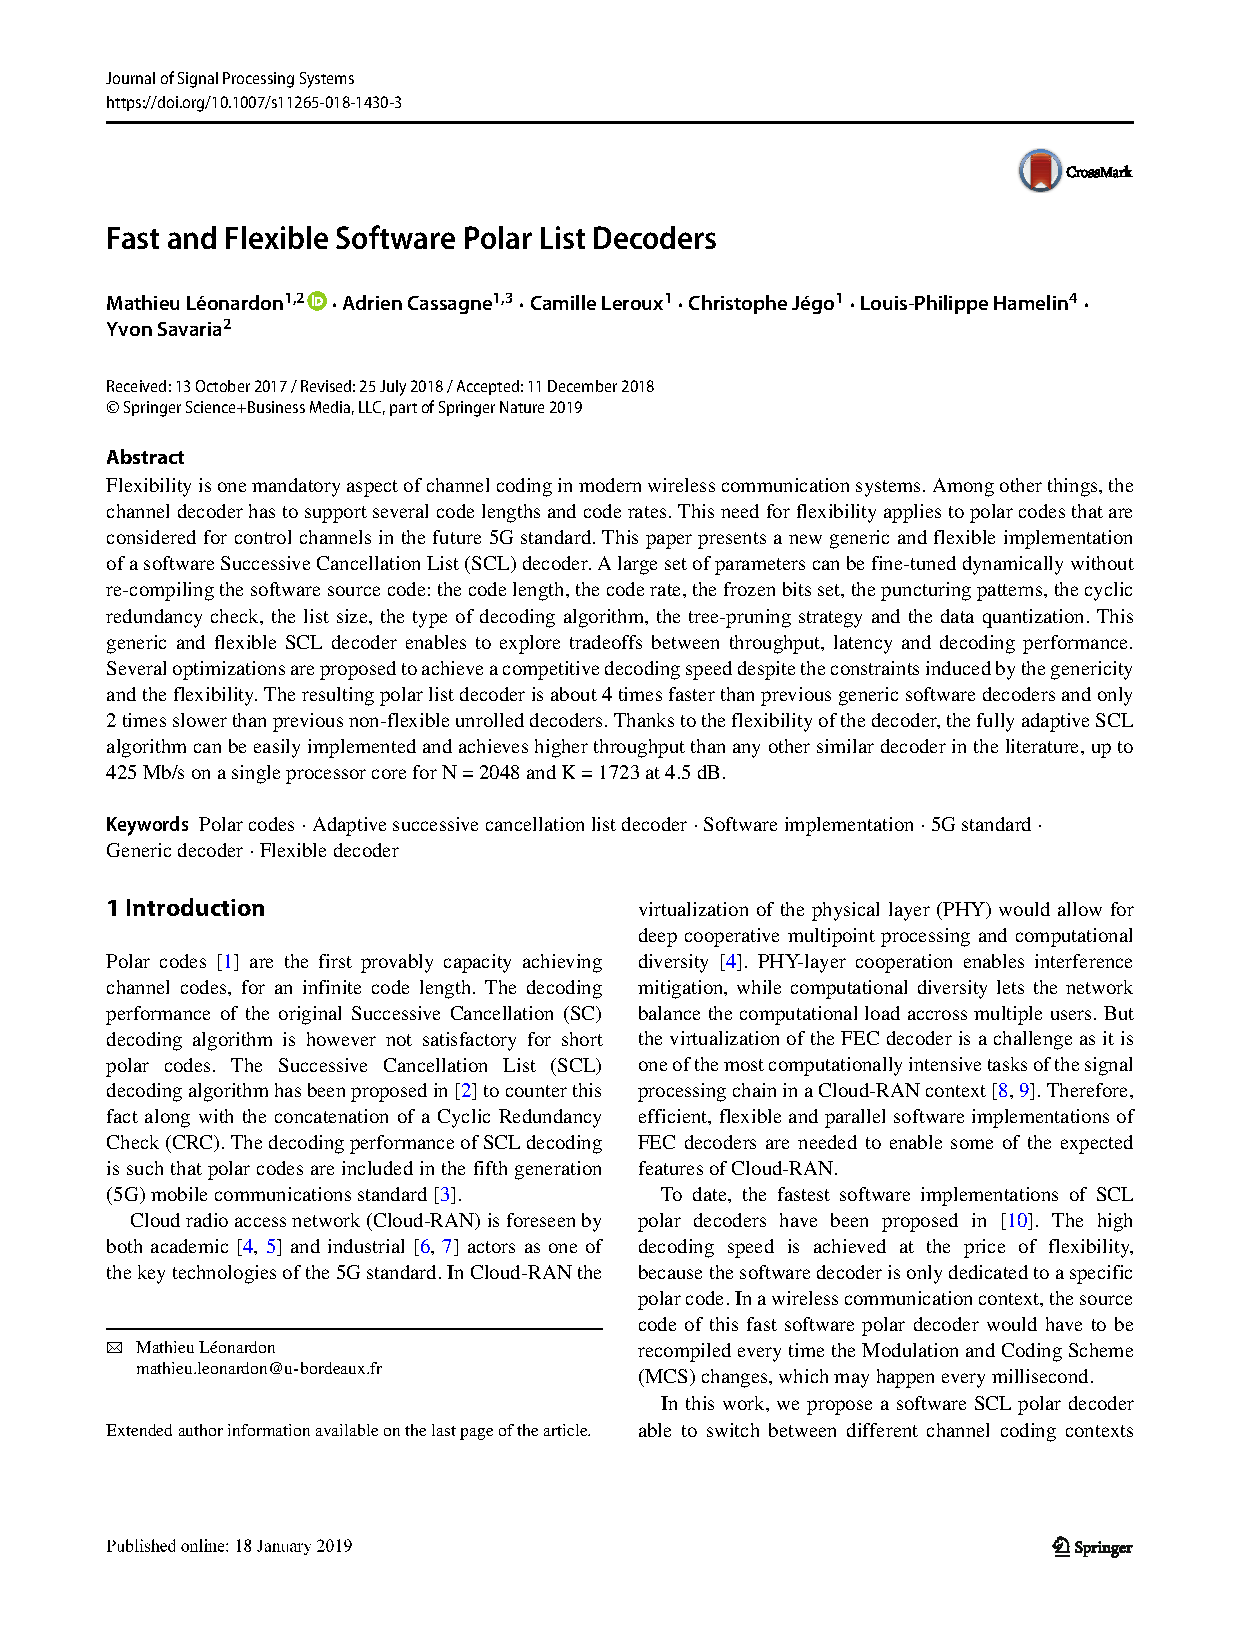
\includepdf[pages=1,pagecommand={\section{Articles}\vspace{1cm}\subsection{Fast and Flexible Software Polar List Decoders}},width=\paperwidth, offset=80 -160]{pieces/article_fast_list.pdf}
\includepdf[pages=2-,pagecommand={},width=\paperwidth, offset=80 -80]{pieces/article_fast_list.pdf}

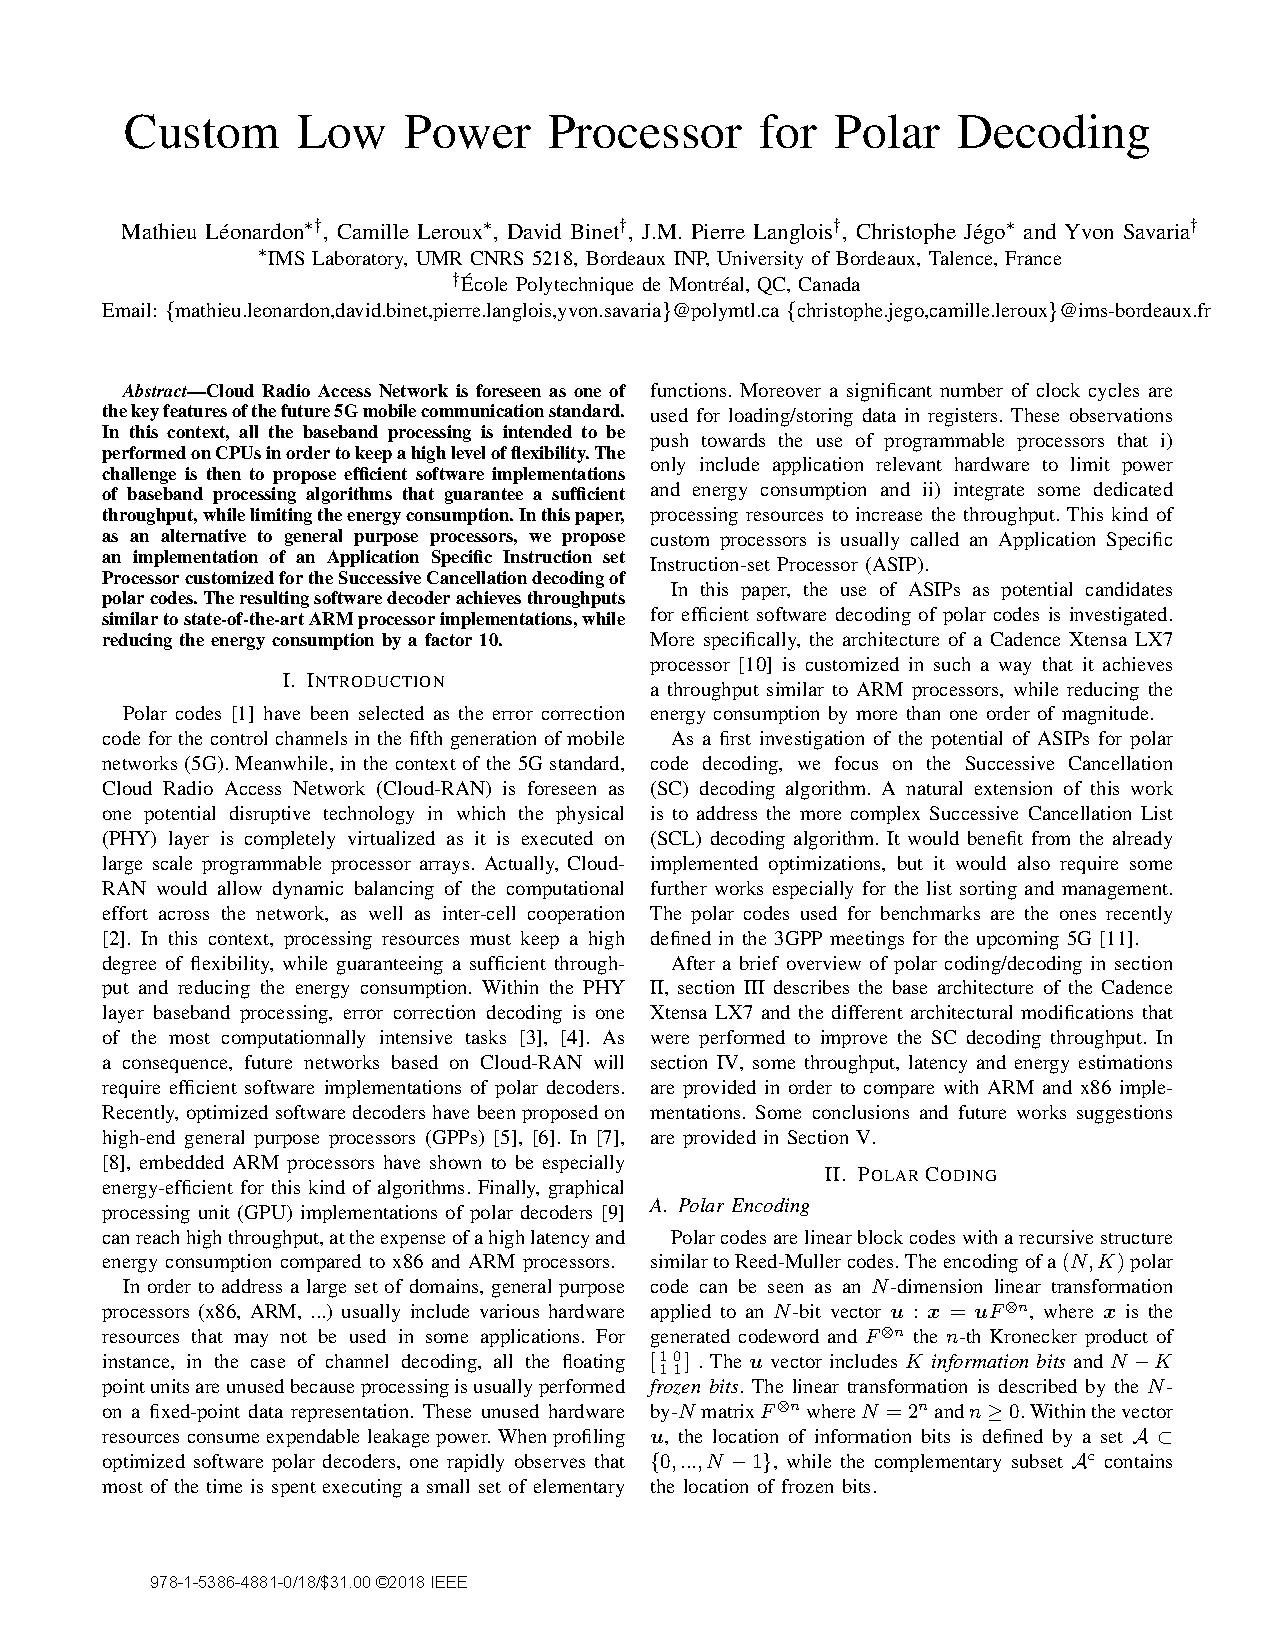
\includepdf[pages=1,pagecommand={\subsection{Custom Low Power Processors for Polar Decoding}},width=\paperwidth, offset=80 -100]{pieces/article_custom.pdf}
\includepdf[pages=2-,pagecommand={},width=\paperwidth, offset=80 -40]{pieces/article_custom.pdf}

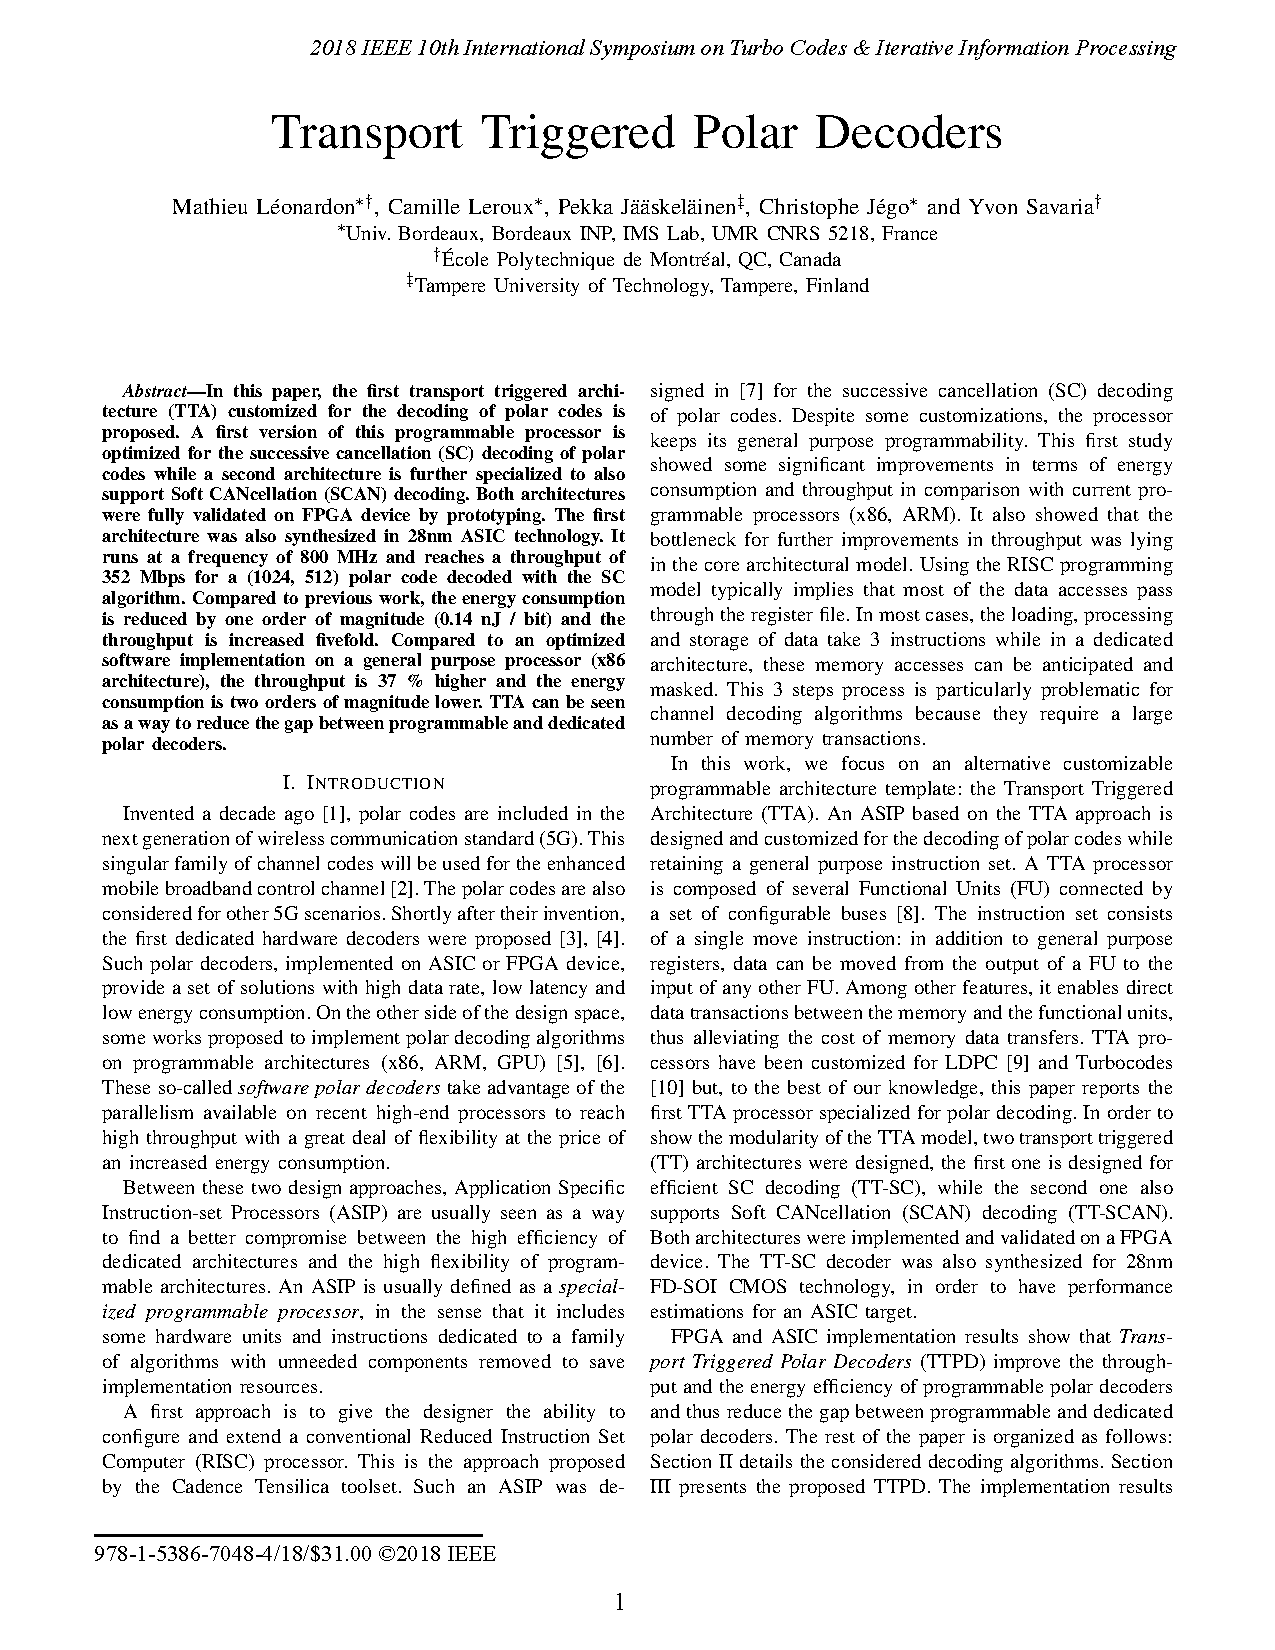
\includepdf[pages=1,pagecommand={\subsection{Transport Triggered Polar Decoders}},width=\paperwidth, offset=80 -135]{pieces/article_ttpd.pdf}
\includepdf[pages=2-,pagecommand={},width=\paperwidth, offset=80 -40]{pieces/article_ttpd.pdf}


\end{document}
